\textit{\emph{•\emph{\textit{•}}}}\section{Design}

\label{Design}

On a normal NFS read the client waits till the server responds with the data. This involves server fetching the data from the slow disk. Thus the client is blocked until the server responds. Instead, NFS asynchronous read responds immediately without blocking the client until the data is ready. Before analysing the two versions of \textsc{NFS reads}, let us take a look at the initial steps performed by the client to acquire the \textit{stateid} required to perform \textsc{read} operation in both the cases. First, the NFS client triggers an \textsc{op\_lookup} request to the server looking for the file. On finding the file the server responds with a \textit{filehandle} back to the client. The client then issues an \textsc{op\_open} on the \textit{filehandle}. On a successful open the server constructs an unique \textit{stateid} and returns it to the client along with the \textit{status}. In case if the file is already opened, then the above mentioned steps are skipped. The \textit{stateid} represents the state information of current \textit{open} request. This state information includes, but is not limited to lock or share state, delegation state. Let us now analyse the sequence of steps involved in \textsc{NFS read} (3.1) and then our asynchronous read using callback mechanism (3.2).

\begin{figure*}
\centering
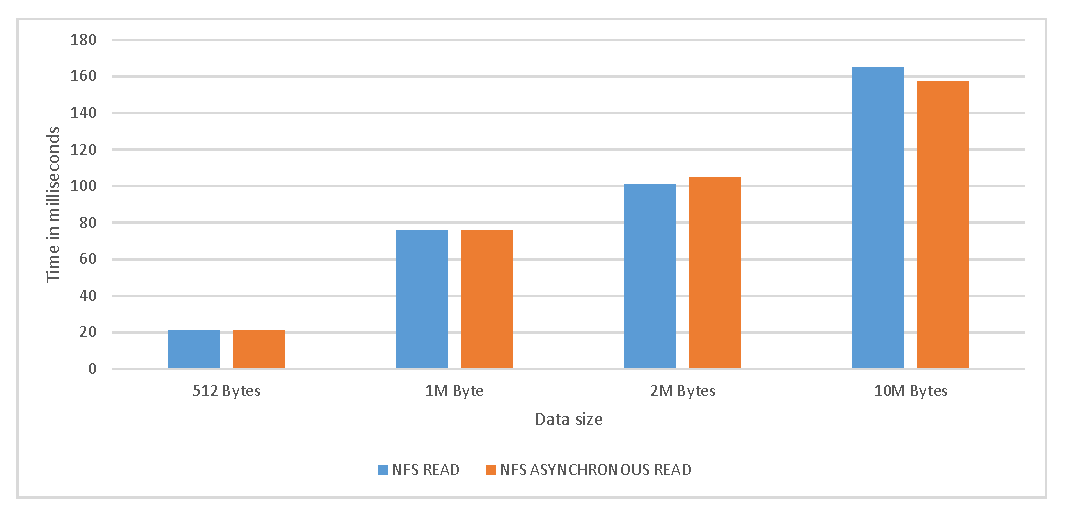
\includegraphics[scale=1.0]{figures/completion_time.eps}
\caption{Completion	Time for NFS Asynchronous read and normal NFS read on a flash storage}
\label{fig:NFSCompletionTimes}
\end{figure*}  

\subsection{NFS READ}
Figure~\ref{fig:NFSRead} depicts the sequence of calls involved in an \textsc{NFS read}. On an existing system, the client uses the same \textit{stateid} in the \textsc{op\_read} request. The server on receiving the request, first checks if the \textit{stateid} is valid. If the \textit{stateid} is invalid, the server responds with a status indicating the \textit{stale stateid}. If valid the server then checks, if the client has acquired the read or share \textsc{read} access while opening the file. Once all the checks are passed, the server then performs read from the local file system or cache. On success the server responds with the \textsc{nfs4\_ok} status along with the data. In case of an error, the server responds with an appropriate error status. Note that the client is blocked until the server responds to the request.

\subsection{Asynchronous Read Using Callbacks}
Figure~\ref{fig:NFSAsyncRead} depicts the sequence of calls involved in an asynchronous read. In the case of asynchronous read, the client first triggers an \textsc{op\_asyncread} operation. The server checks if the \textit{stateid} is valid. It then checks the access permissions on the \textit{stateid} similar to \textsc{op\_read}. Once the checks succeed, the server delegates the request to a new thread and responds back immediately with the status \textsc{nfs4\_ok} without fetching the data from the disk.  Note that this status does not indicate a successful fetch of the data from the disk. We made this decision to avoid any sort of disk access before responding with the initial status. On receiving the initial response, client is not blocked any more and is free to perform further tasks. The new thread created by the server, tries to fetch the data from the disk. On success this thread triggers  \textsc{cb\_async\_read}, a callback to the client. The client on receiving the \textsc{cb\_async\_read} request identifies the request owner based on the \textit{stateid}. Request owner can  be a process or a thread on the client that issued the request. Client on receiving the callback responds with the \textsc{nfs4\_ok} back to the server or an error status if any.  Client on receiving the callback, responds with the \textsc{nfs4\_ok} back to the server or an error status if any. Now on the client side, the process or the thread that has initiated the request can be identified using \textit{session}. But the same thread might have triggered multiple requests. Thus we have added a unique field in the request called \textit{reqid}.  \textit{reqid} enables the process or the thread to uniquely identify the request among the multiple requests that it might have triggered. We also have added an another field named  \textit{timeout} as part of  the asynchronous request to the server. \textit{timeout} is a configurable field that enables the client to specify the maximum time that the server can take to send a callback to the client. If the client does not receive a callback in the mentioned  \textit{timeout}, the client treats the request as a failure and resends the request.

\begin{figure*}
\centering
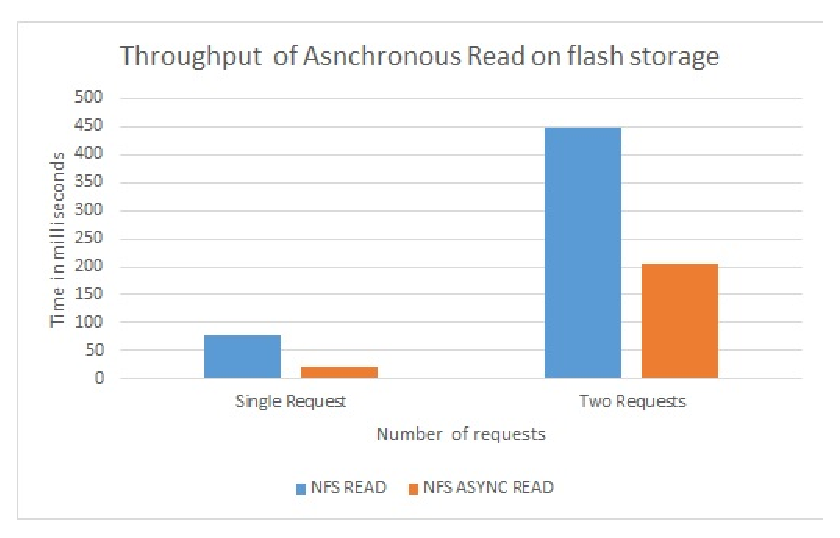
\includegraphics[scale=1.0]{figures/Throughput.eps}
\caption{Throughput for NFS asynchronous read and normal NFS read on a flash storage}
\label{fig:NFSThroughput}
\end{figure*}




%%%%%%%%%%%%%%%%%%%%%%%%%%%%%%%%%%%%%%%%%%%%%%%%%%%%%%%%%%%%%%%%%%%%%%%%%%%%%%
%% For Emacs:
% Local variables:
% fill-column: 70
% End:
%%%%%%%%%%%%%%%%%%%%%%%%%%%%%%%%%%%%%%%%%%%%%%%%%%%%%%%%%%%%%%%%%%%%%%%%%%%%%%
%% For Vim:
% vim:textwidth=70
%%%%%%%%%%%%%%%%%%%%%%%%%%%%%%%%%%%%%%%%%%%%%%%%%%%%%%%%%%%%%%%%%%%%%%%%%%%%%%
% LocalWords:
